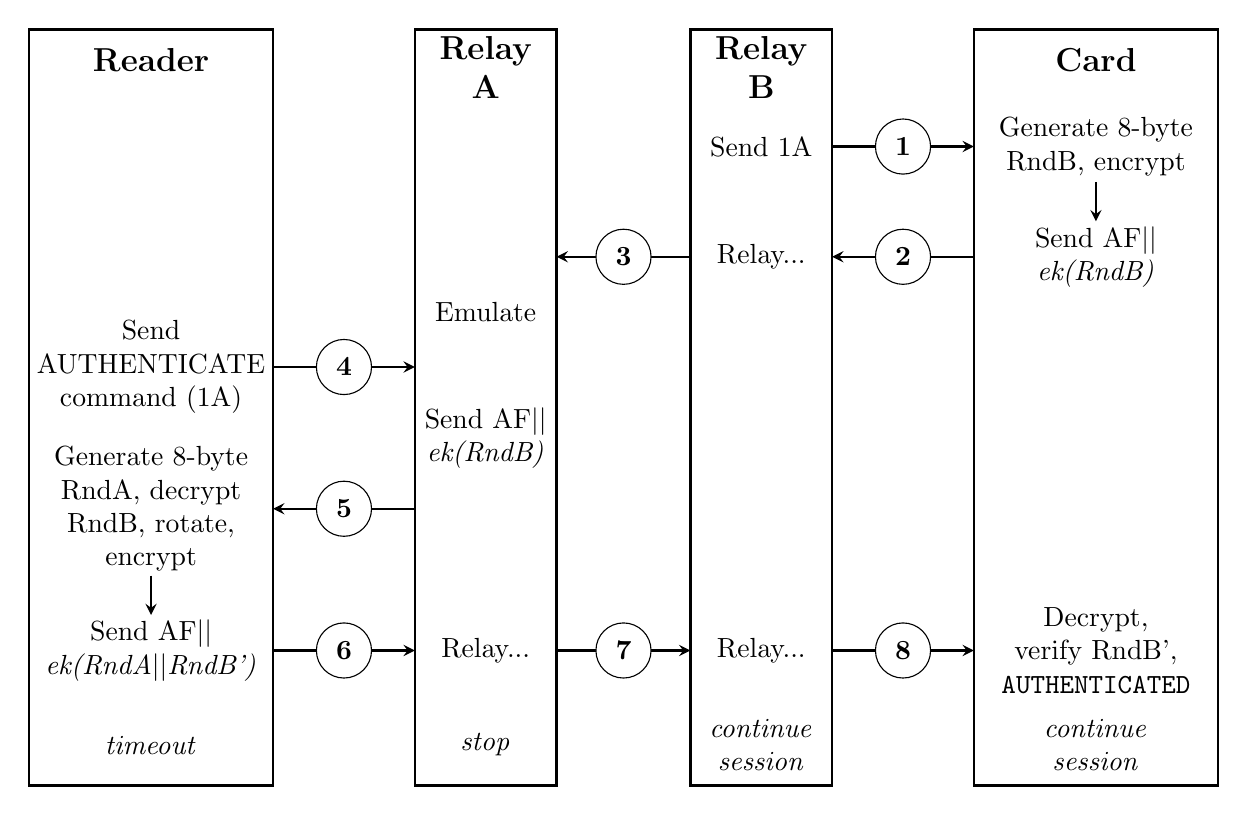
\begin{tikzpicture}[
    % Define styles
    box/.style={
        rectangle, 
        draw, 
        thick,
        minimum width=3.1cm, 
        minimum height=9.6cm,
        anchor=north
    },
    relaybox/.style={
        rectangle, 
        draw, 
        thick,
        minimum width=1.8cm, 
        minimum height=9.6cm,
        anchor=north
    },
    plaintext/.style={
        rectangle, 
        draw,
        thick,
        minimum width=8.1cm, 
        minimum height=0.8cm,
        anchor=north
    },
    arrow/.style={
        ->, 
        >=stealth,
        thick
    },
    numbered/.style={
        circle,
        draw,
        fill=white,
        minimum size=0.7cm,
        font=\bfseries
    }
]

% Set up the coordinate system
\def\yshift{0}
% Variables
\def\readerx{-6}
\def\boxwidth{3.1} % must match style
\def\relaywidth{1.8} % must match style
\def\relayAx{-1.75}
\def\relayBx{1.75}
\def\cardx{6}
\pgfmathsetmacro{\readerxE}{\readerx+\boxwidth/2}
\pgfmathsetmacro{\cardxW}{\cardx-\boxwidth/2}
\pgfmathsetmacro{\relayAxW}{\relayAx-\relaywidth/2}
\pgfmathsetmacro{\relayAxE}{\relayAx+\relaywidth/2}
\pgfmathsetmacro{\relayBxW}{\relayBx-\relaywidth/2}
\pgfmathsetmacro{\relayBxE}{\relayBx+\relaywidth/2}
\pgfmathsetmacro{\midBCx}{(\relayBxE+\cardxW)/2}
\pgfmathsetmacro{\midRAx}{(\relayAxW+\readerxE)/2}
\pgfmathsetmacro{\midABx}{0}
\def\steponey{\yshift+2}
\def\steptwoy{\yshift+0.6}
\def\stepfoury{\yshift-0.8}
\def\stepfivey{\yshift-2.6}
\def\stepsixy{\yshift-4.4}
\def\stepniney{\yshift-5.6}
\pgfmathsetmacro{\stepthreefoury}{(\steptwoy+\stepfoury)/2}
\pgfmathsetmacro{\stepfourfivey}{(\stepfoury+\stepfivey)/2}

% Title
% \node[font=\large\bfseries] at (0,\yshift+4.0) {Relaying MIFARE Ultralight~C Authentication};
%\node[font=\large] at (-2.5,\yshift+4.0) {3-Pass Mutual Authentication};

% Draw reader box
\node[box, fill=none, anchor=north] (reader) at (\readerx,\yshift+3.5) {};
\node[font=\large\bfseries] at (\readerx,\yshift+3.1) {Reader};

% Draw relay A
\node[relaybox, fill=none, anchor=north] (relaya) at (\relayAx,\yshift+3.5) {};
\node[align=center, font=\large\bfseries] at (\relayAx,\yshift+3) {Relay\\A};

% Draw relay B
\node[relaybox, fill=none, anchor=north] (relayb) at (\relayBx,\yshift+3.5) {};
\node[align=center, font=\large\bfseries] at (\relayBx,\yshift+3) {Relay\\B};

% Draw card box
\node[box, fill=none, anchor=north] (card) at (\cardx,\yshift+3.5) {};
\node[font=\large\bfseries] at (\cardx,\yshift+3.1) {Card};

\node[align=center] at (\relayBx,\steponey) {Send 1A};

\draw[arrow] (\relayBxE,\steponey) -- (\cardxW,\steponey) node[midway, above, font=\small] {};
\node[circle, draw, fill=white, minimum size=0.7cm, font=\bfseries] at (\midBCx,\steponey) {1};

\node[align=center] at (\cardx,\steponey) {Generate 8-byte\\RndB, encrypt};

\draw[arrow] (\cardx,\steponey - 0.45) -- (\cardx,\steptwoy + 0.45);

\node[align=center] at (\cardx,\steptwoy) {Send AF\textbar\textbar\\\textit{ek{(}RndB{)}}};

\draw[arrow] (\cardxW,\steptwoy) -- (\relayBxE,\steptwoy) node[midway, below, font=\small] {};
\node[circle, draw, fill=white, minimum size=0.7cm, font=\bfseries] at (\midBCx,\steptwoy) {2};

\node[align=center] at (\relayBx,\steptwoy) {Relay...};

\draw[arrow] (\relayBxW,\steptwoy) -- (\relayAxE,\steptwoy) node[midway, below, font=\small] {};
\node[circle, draw, fill=white, minimum size=0.7cm, font=\bfseries] at (\midABx,\steptwoy) {3};

\node[align=center] at (\relayAx,\stepthreefoury) {Emulate};

\node[align=center] at (\readerx,\stepfoury) {Send\\AUTHENTICATE\\command (1A)};

\draw[arrow] (\readerxE,\stepfoury) -- (\relayAxW,\stepfoury) node[midway, below, font=\small] {};
\node[circle, draw, fill=white, minimum size=0.7cm, font=\bfseries] at (\midRAx,\stepfoury) {4};

\node[align=center] at (\relayAx,\stepfourfivey) {Send AF\textbar\textbar\\\textit{ek{(}RndB{)}}};

\draw[arrow] (\relayAxW,\stepfivey) -- (\readerxE,\stepfivey) node[midway, below, font=\small] {};
\node[circle, draw, fill=white, minimum size=0.7cm, font=\bfseries] at (\midRAx,\stepfivey) {5};

\node[align=center] at (\readerx,\stepfivey) {Generate 8-byte\\RndA, decrypt\\RndB, rotate,\\encrypt};

\draw[arrow] (\readerx,\stepfivey - 0.85) -- (\readerx,\stepsixy + 0.45);

\node[align=center] at (\readerx,\stepsixy) {Send AF\textbar\textbar\\\textit{ek{(}RndA{\textbar}{\textbar}RndB'{)}}};

\draw[arrow] (\readerxE,\stepsixy) -- (\relayAxW,\stepsixy) node[midway, below, font=\small] {};
\node[circle, draw, fill=white, minimum size=0.7cm, font=\bfseries] at (\midRAx,\stepsixy) {6};

\draw[arrow] (\relayAxE,\stepsixy) -- (\relayBxW,\stepsixy) node[midway, below, font=\small] {};
\node[circle, draw, fill=white, minimum size=0.7cm, font=\bfseries] at (\midABx,\stepsixy) {7};

\draw[arrow] (\relayBxE,\stepsixy) -- (\cardxW,\stepsixy) node[midway, below, font=\small] {};
\node[circle, draw, fill=white, minimum size=0.7cm, font=\bfseries] at (\midBCx,\stepsixy) {8};

\node[align=center] at (\cardx,\stepsixy) {Decrypt,\\verify RndB',\\\texttt{AUTHENTICATED}};

\node[align=center] at (\relayAx,\stepsixy) {Relay...};

\node[align=center] at (\relayBx,\stepsixy) {Relay...};

\node[align=center] at (\readerx,\stepniney) {\emph{timeout}};

\node[align=center] at (\relayAx,\stepniney) {\emph{stop}};

\node[align=center] at (\relayBx,\stepniney) {\emph{continue}\\\emph{session}};

\node[align=center] at (\cardx,\stepniney) {\emph{continue}\\\emph{session}};

\end{tikzpicture}
